\section{Introduction}

%In tissues, cells are mainly surrounded by an extracellular matrix (ECM), a soft porous media mixed with interstitial fluid and made up of networks of polymer chains and charged proteins. 
\textit{In vitro} studies have shown that ECM rigidity and shear stresses due to the flow of interstitial fluid can promote malignant phenotypes in a population of initially normal cells, impact on cell proliferation and differentiation \cite{ex3}. Further experiments have shown that tumour development is often associated with a stiffening of the tissue compared to the surrounding healthy one \cite{ex4}. This causes cells to be exposed to higher compressive stresses and the blood vessels to collapse, thus impeding the diffusion of substances in the extra-cellular environment. Hence, numerous therapies are less effective \cite{ecm2}. Based on such evidence, it is now widely accepted that, unlike originally thought, biological process are not simply regulated by biochemical signals but by the complex interplay of mechanical and chemical stimuli.
 
Given the different physical nature and scale of phenomena involved, coupling micro-environment and cell behaviours is a problem of high complexity. This requires understanding processes occurring at different temporal and spatial scales and how they interplay to determine the macroscopic behaviour of a tissue, whether healthy or damaged. Despite experiments probing the micro-scale being possible \cite{viscoporo,afmtest}, these are usually limited to controlled environments in contrast to \textit{in vivo} conditions, where we can instead measure macroscopic properties of tissues. In order to extrapolate information on the environment that cells perceive from the data, we thus need quantitative models able to link the tissue and cellular scale. This requires the development of a theoretical framework able to capture both the biology and physics involved which must also be consistent with the known universal laws of nature \cite{NET}. Having such knowledge can lead to the development of novel therapies that target the cell micro-environment and thus change the current approach to drug design.  

As discussed in Section \ref{ECMcomp}, the ECM is a polyelectrolyte gel \cite{ecm1,ecm2}, i.e. an hydrogel with charged groups. Besides being largely present in the natural world, synthetic polyelectrolytes are currently employed for a wide range of applications, such as drug delivery, biomedical devices, scaffolds for tissue engineering and soft robotics \cite{hydroex3,hydroex2,hydroex1,hydroex4}. Hence, there has been a growing interest in the soft matter community in understanding their behaviour and translating it into mathematical models. In particular, research has been focusing on the phenomena of swelling, i.e. large deformation due to absorption of water, and the diffusion, transport and release of a solution \cite{DROZDOV+,DROZDOVph,Reviewpolyel,swell2}. In these studies, polyelectrolytes are commonly modelled as poro-elastic material. However, with the development of new experimental techniques such as Atomic Force Microscopy (AFM), which test the local mechanical properties of a material, soft tissues and hydrogels have been found to be visco-elastic \cite{ex5}. As their solid skeleton, i.e. polymer network, is deformed, this can change its conformation to a most entropically favourable one thus dissipating energy. Where purely elastic solids deform instantaneously, viscoelastic materials have time-dependent deformation due to the irreversible nature of the process. 

Despite experimental evidence, theoretical studies on visco-elastic soft materials remain limited. Our work aims to develop a continuum mathematical model of the extracellular matrix which is consistent with the laws of thermodynamics and accounts for the poro-visco-elastic nature of ECM. Transport and electro-chemical phenomena due to the flow of interstitial fluid are also included and coupled to the time-dependent deformation of the ECM by the use of linear non-equilibrium thermodynamics. Despite the focus on soft tissues, our results can be more widely applied to the study of polyelectrolyte gels. At our present knowledge, there is no previous work in the literature capturing all these aspects in a non-equilibrium thermodynamics framework. In \cite{ecm1,ecm2} Xue et al.~ develop a nonlinear poroelastic theory for ECM, which couples all three physical phenomena but does not include viscous dissipation. In \cite{Jeru}, the authors couple mechano-electrophysiological effects including the viscous dissipation but neglect transport; Caccavo et al.~ \cite{Article1} propose a poro-viscoelastic model for neutral hydrogel, thus excluding electrical effects.

As discussed in \cite{viscoporo}, there are spatial and time scales which allow us to study visco-elasticity and poro-elasticity independently. On one hand, nanoscale rheological testing with AFM give us information on the visco-elastic properties of the sample. In the case of tissues and hydrogels, the most common rheological model used to fit experimental measurement is the 1D \textit{Standard Linear Solid} model\cite{Article1,viscoporo}, see Figure \ref{SLS}. The poro-elastic behaviour can instead be characterized by standard creep-relaxation test. In this case, Darcy's law is usually applied to estimate the hydraulic conductivity and thus characterise the transport of fluid in the material, which usually modelled as an hyper-elastic solid \cite{Netti,viscoporo}. Even though we have a good understanding of the two phenomena independently, there has been little attention to investigating how the two couple. 

Following a typical approach in the framework of large deformations, we will be using a multiplicative decomposition of the deformation gradient to account for the two phenomena simultaneously. 
Based on previous studies, we here propose two different decompositions. Instead of arbitrarily choosing one of the two, we here develop both approaches with the aim of identifying their differences and investigating how experimental tests can be used to select the most appropriate. At the best of our knowledge, this is the first time the two are systematically compared in the literature.


\begin{figure}
	\begin{subfigure}{0.45\textwidth}
		\centering 
		\def\svgwidth{1.3\linewidth}
		\input{latex/images/SLStand.pdf_tex}
		\caption{}
	\end{subfigure}
	\begin{subfigure}{0.45\textwidth}
	\centering
	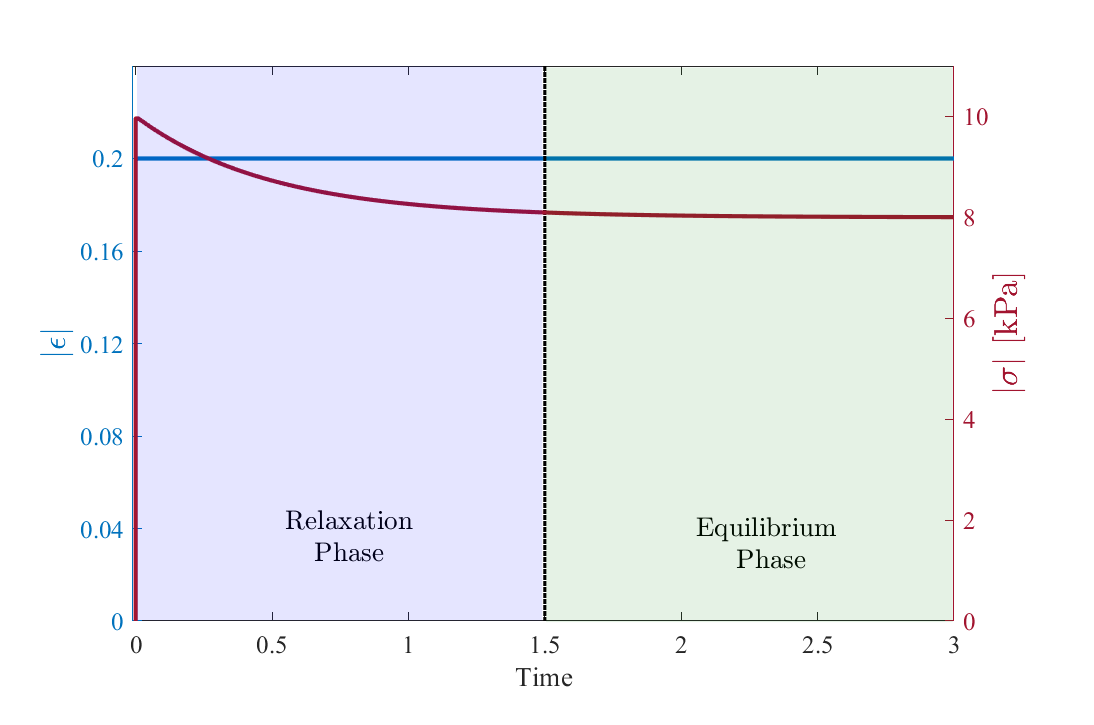
\includegraphics[scale=0.28]{images/SLS}\qquad 
	\caption{}
	\end{subfigure}

\vspace{5mm}
\begin{equation}
\begin{cases}
\sigma = E_1\epsilon+E_2\epsilon_d\\
\dot{\epsilon}_e = \dot{\epsilon} -\frac{E_2}{\eta} \epsilon_e = \dot{\epsilon} - \frac{\epsilon_e}{\tau_R}
\end{cases}
\end{equation}
\vspace{3mm}
\caption{1D Standard Linear Solid. (a) Rheological Model; (b) Standard Response to a compression test. (1) Differential Equation for the Standard Linear Solid model in the 1D case.}
\label{SLS}
\end{figure}

Our work is organized as follows: in Section \ref{ECMcomp}, we discuss more in details the composition of the ECM. We then present a brief overview of Classical Irreversible Thermodynamics, which focuses on the principles later used in Section \ref{modeldev} for the model derivation. Two different approaches to model the kinematics of the deformation are proposed and later compared in Section \ref{eqtest}. As a result of our analysis, we suggest an experimental protocol which can allow us to validate and select the model that better represent the visco-elastic nature of the ECM. 